%% Working draft; target journal to be decided.
%% Built from the htn-coupling stage documents and ENGINE_FINDINGS.md.
\documentclass[preprint,12pt,nopreprintline]{elsarticle}

\usepackage{booktabs}
\usepackage{tabularx}
\usepackage{seqsplit}
\usepackage{amssymb}
\usepackage{amsmath}
\usepackage{url}
\usepackage{tikz}

\begin{document}

\begin{frontmatter}

%% Title (working)
\title{Characterising and extending the Pulse Physiology Engine for hypertensive older adults: population coverage, physiological parameterisation and haemorrhage response}

\author{David Dasa\\[2pt]{\small ORCID: 0009-0007-1535-5962}}


\begin{abstract}
The Pulse Physiology Engine is an open-source, whole-body physiology simulator in wide use across medical education, research, and training, but its default patient envelope was built around a healthy adult reference state. We tested the engine against two older-adult cohort studies, namely the rural South African HAALSI cohort and the English Longitudinal Study of Ageing, and recorded eight engine-level findings, the most consequential of which is that roughly four in five adults with valid measured blood pressure in both cohorts were excluded before any simulation could run. We report the findings, describe extensions to the engine, and demonstrate their physiological consequence through a paired haemorrhage experiment across twenty cohort-derived bodies showing that simulated haemorrhage tolerance was mechanism-sensitive and not ordered by baseline blood pressure within the tested model phenotypes, so that matching pressure alone does not guarantee matching haemodynamic behaviour; the extensions make the Southern African parameter question askable rather than answered.
\end{abstract}

\begin{highlights}
\item Approximately four in five participants with valid measured blood pressure fall outside the engine's baseline pressure envelope in both a South African and an English cohort sample.
\item Eight engine-level findings are recorded, including a baroreflex-gain parameter that controlled adaptation rate rather than reflex sensitivity.
\item A paired haemorrhage experiment across twenty cohort-derived bodies shows that simulated haemorrhage tolerance is mechanism-sensitive and not ordered by baseline blood pressure within the tested model phenotypes, with the direction stable across endpoint thresholds.
\end{highlights}

\begin{keyword}
Pulse Physiology Engine \sep hypertension \sep older adults \sep model characterisation \sep haemorrhage \sep HAALSI \sep ELSA
\end{keyword}

\end{frontmatter}

\section{Introduction}

The Pulse Physiology Engine is an open-source, C++ whole-body physiology simulator maintained by Kitware \cite{pulse,bray2019}. It is used to provide consistent physiology data to medical education, research, and training technologies, including standalone applications, hardware simulators, and sensor interfaces. Its reference patient, a healthy 44-year-old adult male, was built and validated against healthy-adult physiology, and the engine's default patient envelope encodes that population, deliberately and in documented form \cite{pulsepatient}: baseline blood pressures are admissible only in the 90--120\,mmHg systolic by 60--80\,mmHg diastolic box, with additional rules on pulse pressure, age (18--65 years), body mass index (16--30\,kg\,m$^{-2}$), and height.

Two facts about the world make testing this a reasonable and necessary step. First, elevated blood pressure is a leading modifiable cardiovascular risk factor in ageing populations \cite{gbd2019}, and older adults carry the physiology that goes with it: stiffer conduit arteries \cite{mitchell2004}, ventricular remodelling \cite{ganau1992}, reduced and reset baroreflex function \cite{bristow1969,james1996,xie1991}, and altered renal perfusion \cite{schmieder1994}. Second, none of that physiology is represented by a healthy-adult reference state. If the engine cannot admit the measured pressures of older hypertensive adults and cannot represent the mechanisms that produce them, then its usefulness for this population is bounded in ways its users may not know. Testing the engine against older-adult cohorts therefore determines what the tool can and cannot claim for this population.

We used two cohorts. HAALSI (Health and Ageing in Africa: a Longitudinal Study of an INDEPTH community in South Africa) is a community cohort of 5{,}059 adults aged 40 and older in rural Agincourt, Mpumalanga, South Africa, with Wave~1 measured in 2015 \cite{haalsi}. ELSA (the English Longitudinal Study of Ageing) is a national cohort of English adults aged 50 and older, whose Wave~8 nurse visit (2016--17) provides measured blood pressure \cite{elsa}. The two cohorts were chosen deliberately as a Southern African and an English comparator, to test whether any limitations found are specific to one population or are properties of the engine itself. They were not.

\section{Methods}

\subsection{Engine and repository setup}

The tested engine is Pulse 4.3.2 at upstream revision \texttt{e8a36497} (branch \texttt{stable}), with a fork branch (\texttt{public/paper-2026-08-21}) carrying the parameterisation and exposure changes described in Section~\ref{sec:extensions}. Every change was gated by a regression before its results were admitted (Supplementary Material): the distributed \emph{HemorrhageToShock} verification scenario (StandardMale, 30\,s stabilisation, fixed 200\,mL/min bleed for 625\,s, recovery; total simulated time 2{,}155\,s) must leave the archived reference trace unchanged. Within the study's build chain, the gate was byte-identity: any engine change that broke it was rejected regardless of intent, and the archived trace (46{,}098{,}446 bytes; SHA-256 begins \texttt{462c4324\ldots{}fcfab0a}, full value in the Supplementary Material) was reproduced byte-for-byte after every fork commit. Across an independent rebuild on the publication machine (21 August 2026), the same source produces a trace with identical structure (107{,}752 rows) in which 1{,}688 of the numeric cells differ from the archive by at most 0.01 in absolute value (maximum relative deviation below 0.2\%), consistent with build-chain floating-point differences rather than a change in simulated physiology; the public-fork source and the pre-exposure source rebuild to the identical publication-machine hash. The byte-identity guarantee is therefore relative to a fixed build, and the archived reference remains the canonical trace.

\subsection{Cohorts}

HAALSI Wave~1 enrolled 5{,}059 community-dwelling adults aged 40 and older in Agincourt, Mpumalanga, South Africa, in 2015 \cite{haalsi}. Blood pressure was measured in up to three readings per visit; the released derived means (the mean of readings 2 and 3 where available) are non-missing for 4{,}895 participants, and this is the primary denominator throughout. ELSA Wave~8 (2016--17) nurse visits number 3{,}525; ELSA's own validity flag identifies 3{,}317 records with valid mean systolic and diastolic pressure \cite{elsa}. Age, height, and weight were joined from the Harmonized ELSA file. Both are unweighted health-visit samples; neither cohort was selected for blood-pressure extremes. For subgroup analyses, hypertension was operationally defined as systolic pressure $\geq$140 or diastolic $\geq$90\,mmHg, wide-pulse-pressure hypertension as hypertension with pulse pressure $\geq$60\,mmHg, and isolated systolic hypertension as systolic $\geq$140 with diastolic $<$90\,mmHg; a target pressure pair is classed as unreachable when no modifier combination within the calibration domain (systemic resistance multiplier at most 2.0, arterial compliance multiplier at least 0.4) reproduces it within the prespecified $\pm$5/$\pm$5\,mmHg tolerance. The $\geq$140/90\,mmHg threshold is an operational study definition; medication status is not incorporated into the coverage definitions. Three coverage definitions are distinguished throughout: geometric box coverage (systolic 90--120 and diastolic 60--80\,mmHg); complete stock pressure-rule coverage (the box plus the diastolic-to-systolic ratio rule); and full patient-envelope coverage (all hard rules, including age, BMI, and height). Findings 1 and 2 report the first two; the pressure columns of Table~\ref{tab:coverage} report complete stock pressure-rule coverage. Table~\ref{tab:cohort} summarises the analysed samples.

\begin{table}[t]
\centering
\caption{Characteristics of the analysed cohort samples (participants with valid measured pressure). Values are median (interquartile range) unless stated.}
\label{tab:cohort}
\begin{tabularx}{\textwidth}{lXX}
\toprule
 & HAALSI Wave 1 & ELSA Wave 8 \\
\midrule
$n$ & 4{,}895 & 3{,}317 \\
Age (years) & 61.0 (52.0--71.0) & 69.0 (62.0--77.0) \\
Female (\%) & 53.8 & 55.4 \\
Systolic BP (mmHg) & 134.5 (121.5--151.5) & 130.5 (120.0--142.0) \\
Diastolic BP (mmHg) & 81.0 (73.5--90.0) & 72.0 (65.0--79.0) \\
Pulse pressure (mmHg) & 53.0 (44.0--64.5) & 57.5 (49.0--68.0) \\
BMI (kg\,m$^{-2}$) & 26.3 (22.5--31.1) & 27.5 (24.5--30.8) \\
\bottomrule
\end{tabularx}
\end{table}

\subsection{Engine characterisation and counter-testing}
\label{sec:methods-char}

The eight findings of Section~\ref{sec:findings} are the output of a fixed characterisation protocol, applied before any extension was accepted. Its elements are: (i) \emph{boundary testing}: feeding the engine patient values at and just outside each documented admissibility bound and recording whether the response is acceptance, explicit rejection, or silent substitution; (ii) \emph{cohort coverage analysis}: scoring every participant in the two cohorts against each engine rule, alone and jointly, to identify the binding constraints; (iii) \emph{route comparison}: constructing closely matched hypertensive pressures by direct patient initialisation and by cardiovascular modifiers, and comparing the resulting internal states; (iv) \emph{convergence grids}: sweeping target pressures and parameter values through the stabiliser and recording convergence, non-convergence, and stabilisation cost; (v) \emph{parameter perturbation and counter-tests}: varying one exposed parameter at a time, including values chosen to be wrong in a diagnostic direction, and auditing the trajectory rather than only the endpoint; (vi) \emph{trajectory audits}: reading effector scales and state variables along the trajectory to check that a parameter's behaviour matches its claimed semantics; and (vii) \emph{regression verification}: within the fixed study build chain, every engine change must reproduce the archived reference run byte-for-byte. An observation qualifies as an engine finding only when it is reproducible in the tested build, attributable to a specific rule or mechanism, and documented with its evidence. A limitation corrected in the fork is retained as a finding when the correction itself demonstrates a semantic risk that users should carry into other parameters (Finding~8).

\subsection{Haemorrhage experiment}

Twenty HAALSI-derived, engine-admissible bodies (10 per sex, spanning within-sex BMI ranks, ages 40--65; blood pressure was not used for selection) each received four phenotypes under the same fixed haemorrhage: normotensive; resistance-dominant (systemic vascular resistance $\times$2.0); compliance-dominant (arterial compliance $\times$0.4); and combined (both modifiers). Bleeding was fixed at 200\,mL/min from 30 to 655\,s. The primary endpoint is fractional: the time at which mean arterial pressure (MAP) falls 30\% below each run's own baseline (the median over seconds 0--29). The endpoint is fractional rather than absolute because the phenotypes start at different pressures ($\approx$95.2\,mmHg for normotensive, 96.5\,mmHg for compliance-dominant, 120.0\,mmHg for resistance-dominant), and an absolute threshold such as MAP 65\,mmHg confounds distance-to-threshold with mechanism; the fractional endpoint reduces this baseline distance-to-threshold confound and permits comparison of the subsequent dynamics. Endpoints at 20\% and 40\% falls were recorded alongside, and are reported as a sensitivity analysis in Section~\ref{sec:haem-results}.

\section{Engine findings}
\label{sec:findings}

Eight engine-level findings were established over the course of the work; Table~\ref{tab:findings} classifies each by type. They are stated against the tested build and configuration; they are observations of a specific engine, not claims that every use case fails in the same way. Findings 1 and 2 lead because they are the most consequential for anyone trying to use the engine with this population; the remaining six follow in the order they were established.

\paragraph{Finding 1: Baseline pressure admissibility constraint} Stock patient creation enforces a baseline pressure admissibility constraint: any measured pressure outside the 90--120\,mmHg systolic by 60--80\,mmHg diastolic box, and any record whose diastolic exceeds 75\% of systolic, is rejected. The rejection is explicit, not a silent substitution: one-unit-outside test patients (121/73.5, 89/73.5, 114/81, and 114/59\,mmHg) each returned a hard error while an in-range control was accepted. Across the cohorts, 80.76\% of HAALSI and 81.01\% of ELSA adults with valid pressure fall outside the box (Figure~\ref{fig:coverage}). The constraint is a documented design decision: the engine's patient methodology lists the box and the ratio check explicitly, with the stated rationale of excluding hypotension and hypertension \cite{pulsepatient}; what had not been measured before this work is its population consequence. Direct hypertensive initialisation is therefore coverage-limited by design.

\paragraph{Finding 2: Population-envelope exclusions} Pressure is not the only bound. The age ceiling of 65 years excludes 34.95\% of complete HAALSI cases and 66.53\% of ELSA cases; the BMI range 16--30\,kg\,m$^{-2}$ excludes 30.57\% and 31.00\%; the hard height range (4.5--7.0\,ft) excludes 0.13\% of HAALSI, while the documented sex-specific third-to-ninety-seventh percentile range (163--190\,cm male, 151--175.5\,cm female) is enforced only as a warning in the tested build, flagging 17.13\% of HAALSI and 8.37\% of ELSA. Among complete cases, 89.36\% of HAALSI and 93.70\% of ELSA fail at least one hard rule. Pressure is the binding constraint only in the sense that it alone rejects 32.92\% of HAALSI participants who pass every other assessed rule; relaxing one bound does not make the whole population representable.

\paragraph{Finding 3: No native disease history or progression state} The stock operating point carries no representation of hypertension stage or duration. Cardiovascular modifiers produce an acute-onset phenotype: disease duration, vascular remodelling history, and progression are erased by construction.

\paragraph{Finding 4: Default baroreflex accommodation} When a patient restabilises at a raised pressure, the engine returns all four baroreflex scales to approximately unity (0.9983--1.0003 after a 150/90-class restabilisation). The imposed pressure becomes the new accommodated setpoint: unless stateful baroreflex parameters are supplied, the engine treats the new pressure as normal rather than sustaining a corrective reflex output.

\paragraph{Finding 5: Pressure-dependent renal fraction under open-loop adjustment} The baseline-relative \emph{RenalResistanceAdjustmentFraction} moves renal flow in the intended local direction at fixed systemic resistance, but it does not hold renal flow fraction invariant across the pressure domain: in a pressure grid, renal fraction rose from 0.139 at MAP 93.4\,mmHg to 0.170 at MAP 114.8\,mmHg. This is an open-loop controller interacting with systemic and baroreflex feedback, not a coding-sign failure; the parameter is documented as a resistance adjustment rather than a flow target, and no invariant flow target is available.

\paragraph{Finding 6: Route-dependent hypertensive haemodynamics} At closely matched hypertensive pressures, direct patient creation and modifier-route creation produce opposite renal responses: approximately 1.30$\times$ renal flow for the direct route versus 0.61$\times$ for the modifier route, with material divergence in cardiac output and systemic vascular resistance as well. The modifier route agrees with the established-hypertension literature, which documents the transition from a relatively high-output early phenotype to a high-resistance established phenotype \cite{lundjohansen1991}; the direct route produces the hyperkinetic early phenotype instead. The two routes are not interchangeable representations of the same hypertensive patient, and every result must state which route produced it.

\paragraph{Finding 7: Non-monotonic stabilisation manifold} The engine's convergence domain contains holes that are not monotonic in pressure or parameter magnitude: an isolated contractility multiplier of 0.92 fails at 150/90 while the combined preset succeeds; gain 2.0 produces overdrive collapse; and direct pressure-grid cases at 160/90 and 170/100 fail while 180/110 converges. Calibration and preset searches must treat non-convergence as an observed feature of the tested state space, irrespective of whether its underlying cause is numerical or physiological. The engine's documentation acknowledges in general terms that not every combination of parameters within bounds reaches a stable homeostatic starting point \cite{pulsepatient}; the contribution here is the specific map of these holes and their non-monotonicity.

\paragraph{Finding 8: Physiological parameter with numerical-rate semantics (P3)} Before correction, the baroreflex-gain field multiplied both drive and decay increments. A trace audit showed it changed adaptation rate rather than steady-state reflex sensitivity: at 300\,s, gain 0.40 produced heart-rate and resistance scales of 1.435 and 1.238 versus 1.386 and 1.227 at gain 1.0, higher rather than lower, and produced a plausible but misdirected haemorrhage effect (Figure~\ref{fig:p3}). The implementation is corrected (gain now scales drive only; Section~\ref{sec:extensions}), but the defect is retained as a finding rather than treated as a closed bug, because parameter names and literature-derived values cannot be treated as physiological semantics without trajectory and counter-test validation: the defect was invisible to unit tests, plausible in magnitude, and wrong in meaning, and only testing what the parameter claimed caught it.

\begin{table}[t]
\centering
\caption{Summary of the eight engine findings, with their type, principal consequence, and current status. Types: documented admissibility constraint; model form limitation; undocumented model behaviour; route dependence; numerical convergence behaviour; implementation semantic defect. Statuses: \emph{finding only}; \emph{partially addressed} (the underlying limitation remains); \emph{addressed} (the defect is corrected or the bound removed, in the fork).}
\label{tab:findings}
\begin{tabularx}{\textwidth}{lp{3.0cm}p{2.8cm}Xp{2.2cm}}
\toprule
No. & Short name & Type & Consequence & Status \\
\midrule
1 & Baseline pressure admissibility constraint & Documented admissibility constraint & Direct hypertensive initialisation is coverage-limited; explicit rejection, not clamping & Addressed \\
2 & Population-envelope exclusions & Documented admissibility constraints & Age, BMI and height bounds exclude most older adults even after pressure is relaxed & Partially addressed \\
3 & No disease history or progression state & Model form limitation & Chronic phenotypes must be assembled externally; modifiers produce acute-onset states & Partially addressed \\
4 & Default baroreflex accommodation & Undocumented model behaviour & The engine re-absorbs an imposed pressure as its new setpoint & Partially addressed \\
5 & Pressure-dependent renal fraction & Undocumented open-loop interaction & No invariant renal flow target; fraction drifts with systemic pressure & Finding only \\
6 & Route-dependent haemodynamics & Route dependence & Two routes producing closely matched pressures can yield materially different haemodynamics & Finding only \\
7 & Non-monotonic stabilisation manifold & Numerical convergence behaviour & Calibration searches must expect non-convergence as an observed feature & Finding only \\
8 & Gain as adaptation-rate control (P3) & Implementation semantic defect & Plausible, misdirected haemorrhage effects; semantics cannot be assumed from names & Addressed, retained as finding \\
\bottomrule
\end{tabularx}
\end{table}

\section{Extensions}
\label{sec:extensions}

\subsection{Baseline pressure bounds parameterisation}

The fork adds five optional patient fields across six source files: systolic and diastolic minimum and maximum admissible pressures, plus a maximum diastolic-to-systolic ratio. A patient file may now declare an admissible baseline-pressure envelope; values outside Pulse's reference envelope but inside the declared range are accepted with a warning, while omission preserves upstream behaviour exactly, and positive pressures with systolic above diastolic remain non-configurable hard limits. What did not change matters as much as what did: the age, BMI, and hard-height bounds were deliberately left untouched, and the stabiliser still supplies physiology the patient file did not specify. At 150/90, final tissue resistances for bone, fat, gut, liver, and skin are exactly twice their 120/80 values, so direct hypertension is implemented partly by automatic regional resistance tuning; the bounds change itself adds no new physiology.

Coverage under the predeclared 60--200/40--130\,mmHg research envelope (a study configuration, not a proposed new Pulse default) is shown in Table~\ref{tab:coverage}. Wide-pulse-pressure coverage rose from zero to 95.85\% in HAALSI and 99.73\% in ELSA. Pressure is no longer the binding constraint; among pressure-representable participants, the unchanged age ceiling excludes 33.0\% of HAALSI and 65.2\% of ELSA, and the BMI bound excludes 28.9\% and 30.2\%.

\begin{table}[t]
\centering
\caption{Population coverage before and after the bounds parameterisation. ``Full'' coverage additionally requires age, BMI, and height bounds to pass.}
\label{tab:coverage}
\begin{tabularx}{\textwidth}{X>{\centering\arraybackslash}X>{\centering\arraybackslash}X>{\centering\arraybackslash}X>{\centering\arraybackslash}X}
\toprule
Cohort & Pressure before & Pressure after & Full before & Full after \\
\midrule
HAALSI ($n=4{,}895$) & 19.16\% & 98.61\% & 10.07\% & 40.86\% \\
ELSA Wave 8 ($n=3{,}317$) & 18.99\% & 99.85\% & 6.18\% & 21.40\% \\
\bottomrule
\end{tabularx}
\end{table}

The direct-initialisation grid exposed the non-monotonic stabilisation manifold (Finding 7): eight of ten predeclared pressure pairs from 120/80 to 180/110 converged, with 160/90 and 170/100 failing while 180/110 converged, and the largest residual among successes was 1.66\,mmHg systolic and 0.71\,mmHg diastolic. The manifold is recorded here as a documented outcome of the engine, not as a problem this work attempts to solve: calibrating against this engine is navigation of a holey state space, and pretending otherwise would convert an engine property into a user's surprise.

\subsection{Physiological parameter exposure, P1 to P5}

Five exposure paths were pursued, numbered P1--P5. Each is described by what the engine was doing silently, what the literature says, what the exposed parameter now allows, and where its values come from. Each is assessed against a four-level taxonomy: (i) implementation verified; (ii) the parameter behaves in the intended mathematical direction; (iii) the parameter reproduces an accepted physiological relation; and (iv) the parameter is validated against human data. The level achieved is stated explicitly; most extensions here reach levels (i)--(ii), which is recorded rather than implied.

\paragraph{P1: Renal and hepatosplanchnic flow targets (deferred)} The engine was doing silently: nothing enforced any flow-fraction target, and the one available renal adjustment drifts with pressure (Finding 5). The literature says established hypertension is associated with renal hypoperfusion and an age-accelerated decline in renal perfusion \cite{schmieder1994}, and the proposed target was a renal fraction of 0.80--0.90 of the normotensive value. The exposure was not applied: the direct route produced 1.30$\times$ renal flow at 150/90, indicating compensated, mixed behaviour rather than blanket hypoperfusion, while the modifier route produced 0.61$\times$. Imposing a literature target would have masked exactly the route question Finding 6 raises, so P1 remains a documented deferred decision. Its values would in any case have been imported from the literature: neither cohort measures renal flow. Assessment: deferred; no verification level assigned.

\paragraph{P2: Stateful baroreflex resetting} The engine was doing silently: re-absorbing any imposed pressure as the new setpoint, returning baroreflex scales to unity after restabilisation (Finding 4). The literature says chronic hypertension resets the baroreceptor operating point upward, with directional asymmetry and fast and slow components \cite{xie1991,munch1983}. The exposed fields are a chronic midpoint, directional rapid-reset fractions, and fast and slow time constants, with omission retaining upstream accommodation. A pressure-perturbation demonstration verified that the midpoint is stateful rather than fixed: over 1{,}830\,s the logged midpoint followed a falling load, moving from 95.00 to 91.67\,mmHg as MAP moved from 95.32 to 89.51\,mmHg. A held-pressure test after a state-preservation fix demonstrated the upward direction relevant to chronic hypertension: with MAP held near 110--113\,mmHg, the midpoint moved from 95.00 to 102.40\,mmHg over 300\,s. Provenance: literature-informed parameterisation rather than direct measurement. The reset fractions (0.10/0.30) follow experimental rapid-resetting fractions of approximately 9--14\% for upward and 30--34\% for downward pressure changes in chronic hypertension \cite{xie1991}; the fast and slow time constants (120/1{,}500\,s in the preset) are a two-scale approximation, since reported resetting time constants are of the order of minutes \cite{munch1983}. Neither is a cohort measurement. Assessment: level (ii), the parameter behaves in the intended mathematical direction.

\paragraph{P3: Baroreflex gain} The engine was doing silently: its gain field multiplied both drive and decay increments, so it controlled adaptation rate rather than steady-state reflex sensitivity (Finding 8). The literature says baroreflex sensitivity is reduced in established hypertension and in older adults, in physiological units such as ms/mmHg \cite{bristow1969,james1996}. Mapping published physiological sensitivity onto a dimensionless Pulse multiplier with a normotensive baseline of 1.0 is a modelling choice; the work uses a normalised range of 0.40--0.80 with setup warnings outside it. The field is now exposed and corrected so that gain scales the drive increments only and the state-decay term is untouched. A common-time audit at 60\,s shows the corrected ordering: gain 0.40 gives heart-rate and resistance scales of 0.839 and 0.895, gain 1.0 gives 1.048 and 1.022, and gain 2.0 gives 1.614 and 1.628. The additional sentence this parameter requires: what the original implementation actually controlled was update rate: a numerically plausible, literature-valued field whose real semantics were those of an adaptation-rate controller, and which passed every setup test while being wrong about its own meaning. No clamp exists on the effector scales; gain 2.0 remains an overdrive instability rather than a validated physiological response. Provenance: literature-informed normalised scaling range, not a directly measured physiological gain and not cohort-measured. Assessment: levels (i)--(ii): implementation verified and directionally correct; not a validated physiological gain.

\paragraph{P4: Named haemodynamic-stage metadata} The engine was doing silently: representing no disease history or progression state (Finding 3). The literature distinguishes early/borderline, established, and long-standing hypertension by duration-dependent remodelling \cite{lundjohansen1991}. The exposed field names these stages as patient metadata (\texttt{Unspecified}, early/borderline, established, long-standing); \texttt{Unspecified} preserves upstream behaviour, and at this step the labels are provenance only; no behavioural change is attached. Provenance: the metadata labels are modelling categories informed by the natural-history literature on hypertension; they are not clinical guideline stages. The cohorts contain hypertension-related clinical history but no direct measurements of the mechanisms represented by these parameters. Assessment: level (i): labels carried and round-tripped; no behavioural claim attached.

\paragraph{P5: Ventricular controls} The engine was doing silently: offering no ventricular-level exposure, so the ventricular remodelling of hypertension could not be represented. The literature says essential hypertension remodels the left ventricle \cite{ganau1992} and increases left-ventricular elastance, with heterogeneous changes in systolic function and contractility \cite{cohensolal1994}. Two optional multipliers are now exposed for the left-ventricular maximum elastance: chamber end-systolic elastance scales $E_{\mathrm{max}}$, while intrinsic contractility scales the active ($E_{\mathrm{max}} - E_{\mathrm{min}}$) excursion; the first implementation multiplied both fields into $E_{\mathrm{max}}$ and was caught by the same counter-testing discipline that caught P3. Separability is demonstrated by isolated volume ranges of 52.11--138.13\,mL (chamber only), 65.72--147.25\,mL (contractility only), and 55.73--140.83\,mL (combined), demonstrating wiring rather than validation of a clinical pressure--volume relation. Diastolic beta and relaxation-time parameters remain architecture-dependent and are deliberately not guessed. Provenance: elastance and contractility values from the literature; not cohort-measured. Assessment: levels (i)--(ii): wiring verified and directions separable; not validation of a clinical pressure--volume relation.

\subsection{What these extensions do not claim}

Three claims are deliberately not made. First, defaults are not validated for any specific population: the declared 60--200/40--130\,mmHg envelope is a study configuration, not a proposed new Pulse default, and the stock defaults remain unchanged. Second, no preset represents a real patient: the combined ``established'' preset is a mechanism demonstration: it initialised at MAP 121 rather than its nominal 110 and sits on the direct route, which Finding 6 shows is not interchangeable with the modifier route. Third, the Southern African question is exactly what this work cannot answer from existing literature: HAALSI contains no measurements of baroreflex gain, resetting, or ventricular elastance, and the parameter values used here were established in populations that are not Southern African older adults. The extensions remove the engine's structural exclusions and make the question askable; they do not answer it.

\begin{figure}[t]
\centering
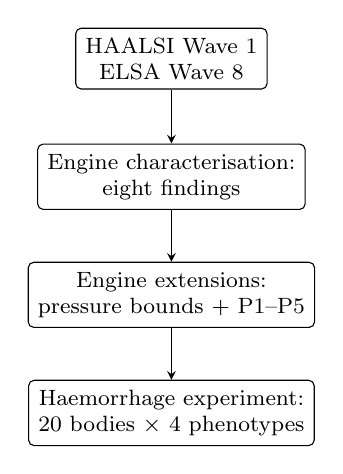
\begin{tikzpicture}[
  every node/.style={draw, rounded corners=2pt, align=center,
                     font=\footnotesize, inner sep=3.5pt},
  >=stealth
]
\node (coh)   at (0,0)    {HAALSI Wave 1\\ ELSA Wave 8};
\node (char)  at (0,-1.5) {Engine characterisation:\\ eight findings};
\node (ext)   at (0,-3.0) {Engine extensions:\\ pressure bounds + P1--P5};
\node (exp)   at (0,-4.5) {Haemorrhage experiment:\\ 20 bodies $\times$ 4 phenotypes};
\draw[->] (coh)  -- (char);
\draw[->] (char) -- (ext);
\draw[->] (ext)  -- (exp);
\end{tikzpicture}
\caption{Study architecture. Two older-adult cohorts feed an engine characterisation protocol, whose findings motivate targeted extensions; a paired haemorrhage experiment across twenty cohort-derived bodies then tests whether mechanism representation matters for simulated tolerance.}
\label{fig:architecture}
\end{figure}

\begin{figure}[t]
\centering
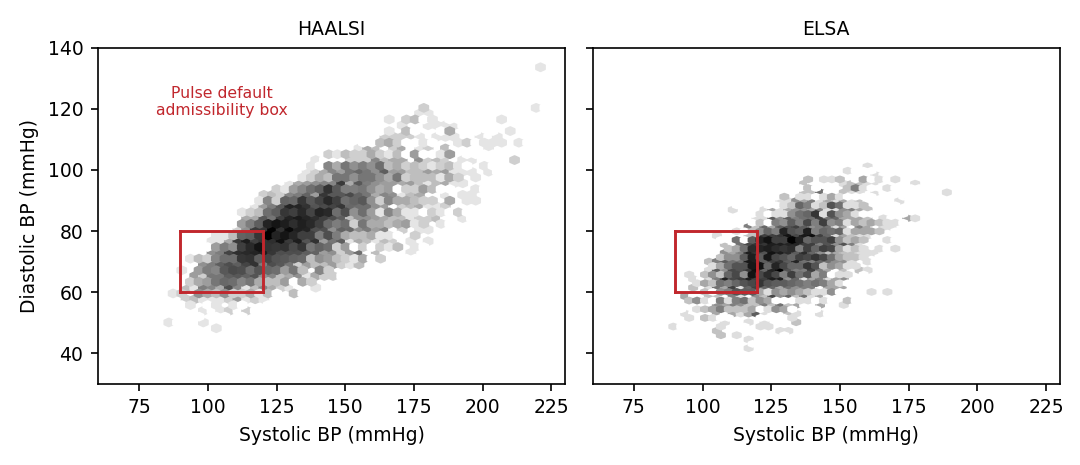
\includegraphics[width=0.9\textwidth]{fig_coverage.png}
\caption{Measured blood pressure in the two cohorts against the engine's default admissibility box (red rectangle, 90--120 systolic by 60--80\,mmHg diastolic). Hexagonal density bins are the HAALSI Wave~1 derived means ($n=4{,}895$) and the ELSA Wave~8 valid means used throughout the analysis ($n=3{,}317$); darker bins mark higher density.}
\label{fig:coverage}
\end{figure}

\begin{figure}[t]
\centering
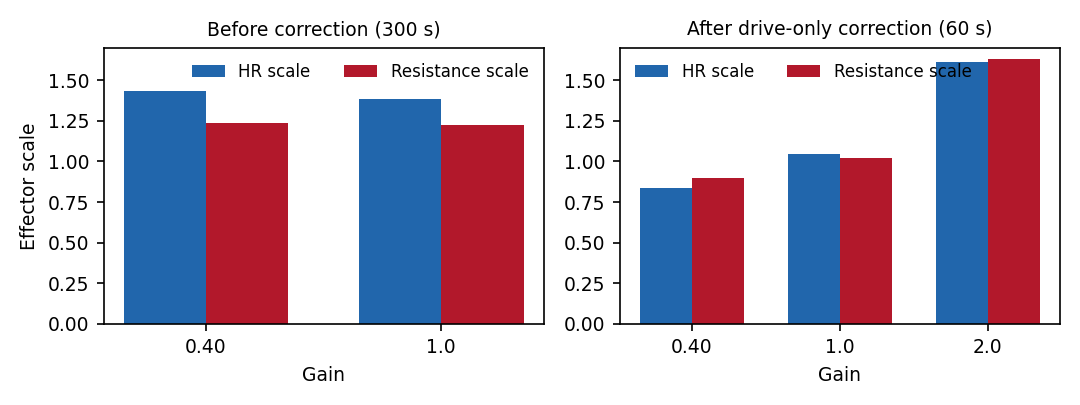
\includegraphics[width=0.9\textwidth]{fig_p3.png}
\caption{The baroreflex-gain trace audit. Left: before correction, gain 0.40 produced \emph{higher} effector scales than gain 1.0 at 300\,s; the field was changing adaptation rate, not reflex sensitivity. Right: after the drive-only correction, effector scales increase monotonically with gain at 60\,s, the ordering a reflex-sensitivity parameter should show.}
\label{fig:p3}
\end{figure}

\section{Haemorrhage experiment}

\subsection{Results}
\label{sec:haem-results}

All 80 runs yielded the primary endpoint. Table~\ref{tab:results} reports the prespecified fractional endpoint (time to a 30\% fall from each run's own baseline MAP), and Figure~\ref{fig:trajectories} shows the median trajectories of MAP and three secondary variables.

\begin{table}[t]
\centering
\caption{Paired haemorrhage results across 20 HAALSI-derived bodies. Endpoint: time to a 30\% fall from each run's own baseline MAP. Paired differences are per body, against the normotensive control of the same body; IQR is the interquartile range of the per-body paired differences.}
\label{tab:results}
\begin{tabularx}{\textwidth}{lp{2.2cm}p{2.8cm}Xp{2.6cm}}
\toprule
Phenotype & Median endpoint (s) & Paired median difference (s) & IQR of paired differences (s) & Direction across 20 bodies \\
\midrule
Normotensive & 481.0 & n/a & n/a & n/a \\
Resistance-only & 416.0 & $-57.0$ & $-63.0$ to $-41.0$ & earlier 20/20 \\
Compliance-only & 487.5 & $+7.0$ & $+6.2$ to $+8.0$ & later 20/20 \\
Combined & 428.5 & $-49.5$ & $-56.0$ to $-37.3$ & earlier 20/20 \\
\bottomrule
\end{tabularx}
\end{table}

Relative to control, resistance-only reached the endpoint 11.9\% earlier, combined 10.3\% earlier, and compliance-only 1.5\% later. No hypothesis tests are reported. The twenty bodies are deliberately selected and the engine is deterministic, so there is no stochastic sampling model under which a $p$-value would have meaning; the evidential weight rests on the direction of the paired difference, which was identical in all twenty bodies for every phenotype, and on its consistency within both sex strata (female paired medians $-55$, $+7$, $-48$\,s; male $-61.5$, $+7.5$, $-54.5$\,s).

The ordering is stable across endpoint definitions. At a 20\% fall from baseline, paired medians were $-57.5$\,s (resistance-only), $+8.0$\,s (compliance-only), and $-49.5$\,s (combined), each earlier/later in 20/20 bodies; at a 40\% fall, $-58.5$\,s, $+7.0$\,s, and $-51.0$\,s, again 20/20 (Figure~\ref{fig:sensitivity}). The qualitative ordering at the prespecified 30\% endpoint is therefore not an artifact of threshold choice.

The median trajectories (Figure~\ref{fig:trajectories}) show that the phenotypes are distinguished by how they compensate, not by where they end: at the end of the bleed, median MAP converges near 42\,mmHg in all four phenotypes. The resistance-carrying phenotypes hold that pressure with vasoconstriction while cardiac output collapses (median 1.00 and 0.95\,L/min at end-bleed, versus 1.87--1.88\,L/min in the compliance-dominant and normotensive bodies), and they mount a smaller peak heart-rate response during the bleed (142 and 137/min, versus 148/min compliance-dominant).

\begin{figure}[t]
\centering
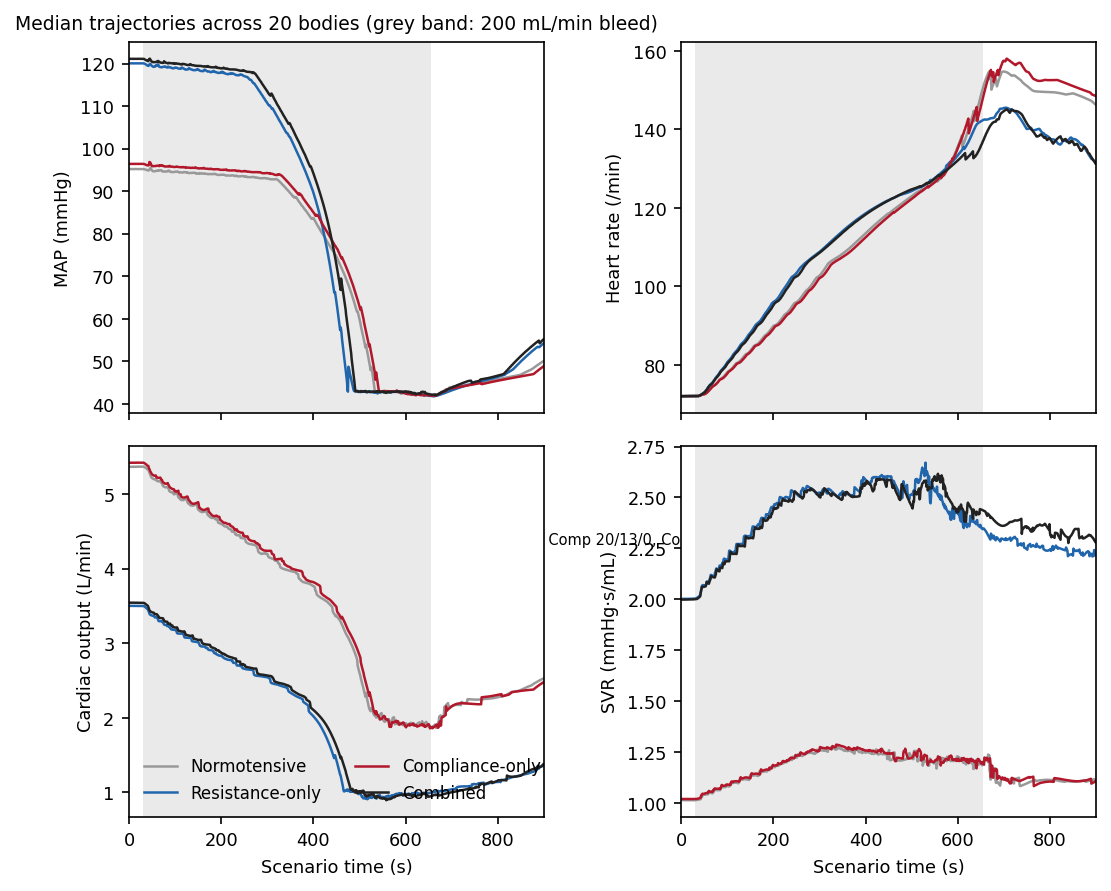
\includegraphics[width=\textwidth]{fig_trajectories.png}
\caption{Median trajectories across the 20 bodies by phenotype (grey band: 200\,mL/min bleed from 30 to 655\,s). Top left to bottom right: MAP, heart rate, cardiac output, and systemic vascular resistance. Runs that reached irreversible state stop contributing beyond their recorded end; the number of active runs at 300/600/900\,s is shown beneath the MAP panel, so the late medians are read against a known denominator.}
\label{fig:trajectories}
\end{figure}

\begin{figure}[t]
\centering
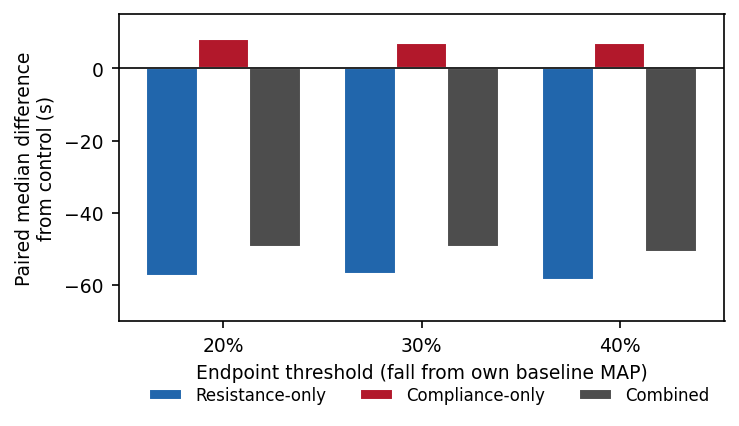
\includegraphics[width=0.7\textwidth]{fig_sensitivity.png}
\caption{Endpoint-threshold sensitivity. Paired median difference from control (s) at 20\%, 30\%, and 40\% falls from each run's own baseline MAP. The direction was identical in all 20 bodies at every threshold.}
\label{fig:sensitivity}
\end{figure}

\subsection{Interpretation}

Two mechanisms, opposite directions, and the ordering of outcomes is not the ordering of pressures. The resistance-dominant phenotype, the one with the worse pressure reading (MAP 120.0\,mmHg), reached the endpoint 57\,s earlier than control in every one of the twenty bodies. The compliance-dominant phenotype, whose MAP of 96.5\,mmHg sits within 1.3\,mmHg of the control's 95.2\,mmHg, reached it 7\,s later in every body. Within the tested model phenotypes, the result is mechanism-sensitive and not ordered by baseline blood pressure: the resistance-dominant phenotype reaches the endpoint earlier, whereas the compliance-dominant phenotype reaches it later, and the phenotype whose baseline pressure is least informative about the simulated endpoint is the one in which the underlying haemodynamic mechanism differs most. The trajectory evidence localises the difference to compensation rather than to the final absolute pressure: the resistance-carrying phenotypes sustain pressure by vasoconstriction while flow support collapses and heart-rate compensation stays modest, whereas the compliance-dominant phenotype preserves cardiac output and reaches a higher peak heart rate.

The phenotype whose simulated haemorrhage endpoint is least predictable from its baseline pressure is also the one the engine represents least well. Wide-pulse-pressure hypertensives were the least representable subgroup within the calibration domain: only 18.5\% of HAALSI and 27.8\% of ELSA wide-pulse-pressure hypertensives were reachable. Reachability is domain-dependent: overall hypertensive reachability is 16.0\%/10.0\% in the original prescribed modifier domain, 29.3\%/35.0\% in the calibration domain used here, and 91.8\%/98.5\% under an unrestricted engineering hull (resistance up to 6.0, compliance down to 0.1) that is numerical reachability rather than physiology; thus the wide-pulse-pressure deficit is reported against the prespecified calibration domain, not the engine's numerical envelope. Among unreachable isolated-systolic cases, the median pulse pressure was 79.5\,mmHg in both cohorts. Compliance enters the engine only as a lumped multiplier. Whether that correspondence reflects arterial buffering physiology or the lumped representation is left open here: the experiment establishes the coincidence, not the mechanism behind it.

\subsection{Limitations}

The bodies are selected (BMI-stratified, age-restricted, engine-admissible) rather than population-representative. The bleed is fixed in absolute mL/min rather than scaled to body size. The engine is deterministic, so no hypothesis testing is reported, and the marked inter-individual differences in hypovolaemia tolerance documented in human studies \cite{xiang2018} enter this panel only through the fixed set of bodies. Compliance is a lumped multiplier with a first-order mapping into the model, not a vessel-resolved stiffness distribution. Per-second trajectories were retained for the panel and summarised as body medians; runs that reached irreversible state stop contributing beyond their recorded end. The result is a mechanism-sensitive engine finding, not a clinical estimate of haemorrhage tolerance.

\section{Discussion}

The headline exclusion is not a Southern African problem. Approximately four in five participants with valid measured pressure fall outside the engine's pressure envelope in the South African sample and in the English sample, within a quarter of a percentage point of each other. The cross-cohort replication demonstrates that the coverage problem is not confined to HAALSI and is consistent with a model envelope problem rather than a property of either population; the fix belongs to the engine's envelope, not to any refinement of our understanding of either population. It is the difference between ``the model does not yet represent these patients'' and ``these patients are somehow special.''

The eight findings share a structure. Each is a case of the engine encoding a physiological assumption as an operating definition: that admissible pressures lie in a healthy-adult box, that the baroreflex should adopt whatever pressure it is given, that a named ``gain'' means reflex sensitivity. Finding 1 differs from the rest in provenance, not in kind: its bounds are published, with the stated rationale of excluding hypotension and hypertension \cite{pulsepatient}, so the contribution there is not exposing a hidden constraint but measuring the population consequence of a declared one, which the documentation never quantifies. Findings 4--8 concern behaviours that remain undocumented. The P3 defect is the sharpest example of the class. A parameter with a literature-derived value, a physiological name, and numerically plausible behaviour meant something different from what it claimed: it set the rate at which the reflex adapted, not the sensitivity of the reflex, and it was found only by testing what it claimed rather than whether it produced an effect. That is the standard the characterisation protocol of Section~\ref{sec:methods-char} encodes, a standard that generalises beyond Pulse to any simulator whose admissibility rules and parameter semantics are inherited, or documented without measured consequence (an audit framework for physiological simulators whose parameters must earn their names), demonstrated here on the authors' own code: the same discipline later caught the authors' first P5 implementation making the same class of error, multiplying two independent fields into one.

The direction this implies is one the engine's own documentation has already named: its patient methodology describes translating personalised physiological profiles, from sources such as electronic health records or wearable sensors, into engine parameters as the route to clinical use, while listing no planned near-term additions \cite{pulsepatient}. The parameterisation work reported here is an instance of exactly that translation, performed at the level of a population rather than an individual. Three things remain open. The Southern African parameter values: whether baroreflex gain, resetting, or ventricular elastance differ in this population is not answerable from existing literature, and this work deliberately does not pretend otherwise. The stiff-artery patient: wide-pulse-pressure hypertensives remain the worst-covered and least-mechanistically-represented group, and the direct and modifier routes still disagree about what they are. The mechanism decomposition: the trajectory evidence shows which components carry the between-phenotype differences, cardiac output preservation and heart-rate compensation, but a per-component attribution of the haemorrhage tolerance difference, together with an exactly pressure-matched direct-versus-modifier grid, is the immediate next step.

\section{Conclusion}

Pulse's stock envelope excludes most participants with valid measured pressure in these older-adult cohorts by design, not by population: the same four-in-five rejection appears in a rural South African cohort and in an English ageing cohort. The extensions reported here address the exclusion and expose the implicit assumptions: the parameterised envelope, the stateful baroreflex, the corrected gain, and the ventricular controls. The haemorrhage experiment shows that simulated tolerance is mechanism-sensitive and is not ordered by baseline pressure within the tested model phenotypes, demonstrating why pressure alone is insufficient to define hypertensive physiology within the model; the extensions make the Southern African parameter question askable, not answered.

\section{Data and code availability}

The characterisation, analysis, and figure-generation scripts, all configuration files, the phenotype definitions, the audited cohort variable mappings, and the result tables cited in the Supplementary Material are retained in the analysis repository \url{https://github.com/Naijaoracle/htn-coupling} (tag \texttt{paper-2026-08-21}). The legacy four-body acute-panel configuration is participant-linked and is retained privately; an example schema is shipped in the repository. The per-body parameter records and the per-run haemorrhage trajectories are participant-linked derivatives and are retained in the private archive only: authorised users regenerate the twenty-body panel and its trajectories from their own cohort copy with the pipeline scripts in the repository (\texttt{scripts/run\_stage5\_expanded\_acute.py}). Cohort data are third-party: HAALSI Wave~1 is available from the HAALSI data platform (ICPSR 36633) and ELSA Wave~8 from the UK Data Service (study 5050); per-participant data are not redistributed; only aggregate statistics and rendered figures appear in the repositories. The engine fork is available at \url{https://github.com/Naijaoracle/pulse-physiology-engine}, branch \texttt{public/paper-2026-08-21} (tag \texttt{paper-2026-08-21}), retaining ancestry from the public upstream revision \texttt{e8a36497} (Pulse 4.3.2, branch \texttt{stable}); its head commit is \texttt{7cad6123e59f583f97a7d9a55568960562adb04c}. The full SHA-256 regression checksum is recorded in the Supplementary Material; an independent rebuild of the public fork on 21 August 2026 reproduced the trace with 1{,}688 numeric cells differing from the archive by at most 0.01 in absolute value (consistent with build-chain floating-point differences; see Supplementary Material).

\appendix

\section{Supplementary material}

\subsection{The eight findings in full technical detail}

\textbf{1. Baseline pressure admissibility constraint.} Stock patient creation rejects any measured adult pressure outside the declared baseline envelope of 90--120\,mmHg systolic by 60--80\,mmHg diastolic; a record whose diastolic exceeds 75\% of systolic is rejected by the pulse-pressure rule. Direct hypertensive initialisation is therefore coverage-limited. A real-engine boundary test accepted the in-range 114/73.5\,mmHg control and returned an explicit error for each one-unit-outside test (121/73.5, 89/73.5, 114/81, 114/59\,mmHg); no log mentioned clamping. The operational finding is exclusion, not silent substitution. In the cohorts, the ratio rule alone fails 31 of 4{,}895 HAALSI records (0.63\%) and 12 of 3{,}317 ELSA records (0.36\%), including four HAALSI records inside the pressure box. The bound is documented in the engine's patient methodology, with the stated rationale of excluding hypotension and hypertension \cite{pulsepatient}; this work measures its population consequence.

\textbf{2. Population-envelope exclusions.} Age (18--65 years), BMI (16--30\,kg\,m$^{-2}$), height (hard range 4.5--7.0\,ft), and pulse-pressure rules exclude additional real-cohort adults. On HAALSI participants complete on pressure, age, sex, height, and weight ($n=4{,}635$): pressure rules reject 80.65\%, BMI 30.57\%, age 34.95\%, hard height 0.13\%; at least one rule rejects 89.36\%. ELSA (complete cases $n=3{,}254$): at least one hard rule rejects 93.70\%; 66.53\% of complete ELSA cases exceed the age ceiling versus 34.95\% in HAALSI. On height, the documented sex-specific third-to-ninety-seventh percentile range (163--190\,cm male, 151--175.5\,cm female) is enforced as a warning in the tested build, flagging 17.13\% of HAALSI and 8.37\% of ELSA; the hard rejection range is the looser 4.5--7.0\,ft, excluding 0.13\% of HAALSI and none of ELSA. The hard-rule percentages reported here therefore use the enforced rejection bound, not the documented percentile bound. Relaxing one bound does not make the whole population representable.

\textbf{3. No native disease history or progression state.} Hypertension stage and duration are not represented as patient history in the stock operating-point definition; modifiers applied at time zero produce acute-onset states in which disease duration and remodelling history are erased by construction.

\textbf{4. Default baroreflex accommodation.} Stock restabilisation returns the baroreflex scales to approximately unity, implicitly treating the new pressure as the normal setpoint unless stateful parameters are supplied. After a 150/90-class restabilisation, baroreceptor heart-rate, elastance, resistance, and compliance scales read 0.9983, 0.9999, 0.9991, and 1.0003.

\textbf{5. Pressure-dependent renal fraction under open-loop adjustment.} The baseline-relative RenalResistanceAdjustmentFraction moves renal flow in the intended local direction at fixed systemic resistance but does not hold the renal flow fraction invariant across the pressure domain. In the pressure grid, renal fraction rose from 0.139 at MAP 93.4\,mmHg to 0.170 at MAP 114.8\,mmHg (grid: resistance multiplier 1.0/1.2/1.4/1.6/2.0). This is an open-loop controller interaction with systemic/baroreflex feedback, not a coding-sign failure; the parameter is documented as a resistance adjustment rather than a flow target. Evidence: \path{results/stage7/p1_target_sweep_final/}, \path{results/stage7/p1_pressure_grid/}, \path{results/stage7/p1_runtime_smoke/}.

\textbf{6. Route-dependent hypertensive haemodynamics.} At closely matched hypertensive pressures, direct patient creation and modifier-route creation produce opposite renal responses: approximately 1.30$\times$ renal flow for the direct route versus 0.61$\times$ for the modifier route (modifier cells not exactly pressure-matched; residuals retained). Direct route cardiac output 5.98--6.44\,L/min and SVR 0.974--0.999\,mmHg\,s\,mL$^{-1}$ versus modifier 4.41--5.26\,L/min and 1.123--1.495; every recorded regional flow separated in the same direction. The modifier route agrees with the established-hypertension literature, which documents the transition from a relatively high-output early phenotype to a high-resistance established phenotype \cite{lundjohansen1991}; direct creation produces the hyperkinetic early phenotype. The two routes are not interchangeable representations of the same hypertensive patient. Both routes reproduced their shared targets within the prespecified $\pm$5/$\pm$5\,mmHg acceptance tolerance, so residual pressure mismatch is bounded by that tolerance, whereas the renal-flow ratio differs by more than a factor of two in opposite directions; an exactly pressure-matched grid remains to be run.

\textbf{7. Non-monotonic stabilisation manifold.} The convergence domain has holes that are not monotonic in pressure or parameter magnitude: an isolated contractility multiplier of 0.92 fails at 150/90 while the combined preset succeeds; gain 2.0 produces overdrive collapse (517--519\,s pre-correction; 74\,s corrected); pressure-grid cases at 160/90 and 170/100 fail while 180/110 converges. The $R=8.0$, $C=0.5$ probe remained CPU-active after 15\,min 41\,s and $>$5{,}000 simulated stabilisation seconds and was operator-censored as non-convergence. Calibration and preset searches must treat non-convergence as an observed feature of the tested state space, irrespective of whether its underlying cause is numerical or physiological. The engine's documentation acknowledges in general terms that not every combination of parameters within bounds reaches a stable homeostatic starting point \cite{pulsepatient}; the contribution here is the specific map of these holes and their non-monotonicity.

\textbf{8. Physiological parameter with numerical-rate semantics (P3).} Before the drive-only correction, the baroreflex-gain field multiplied both drive and decay increments. Trace audit at 300\,s: gain 0.40 produced HR/resistance scales 1.435/1.238 versus 1.386/1.227 at gain 1.0. Since gain multiplied both the state decay and the drive increments, it changed update rate rather than steady-state reflex sensitivity, producing a plausible but misdirected haemorrhage effect. The implementation is corrected (gain scales drive only), but the defect remains an engine-development finding: parameter names and literature-derived values cannot be treated as physiological semantics without trajectory and counter-test validation.

\textbf{Supplementary observation: Aorta-InFlow morphology.} Pulse's lumped Aorta-InFlow lacks the brief post-ejection reverse-flow feature of physiological aortic flow around valve closure, and is lower-peaked, lower-volume, and longer relative to its cycle than a distributed reference inlet (peak flow 434.75 versus 572.73\,mL/s; stroke volume 80.35 versus 112.90\,mL; post-peak minimum flow approximately 0 versus $-162.89$\,mL/s). On identical distributed-network geometry and published terminals, substituting the Pulse inlet lowered aortic pulse pressure by 13.84\,mmHg (34.41 to 20.57\,mmHg); the coupled aortic pulse pressure of 20.45\,mmHg is below the 31.2\,mmHg age-45 mean of a healthy-ageing reference database \cite{charlton2019}. Pulse does not claim that this compartment-flow trace is a validated physiological aortic waveform, so this is a scope observation rather than a validation failure; it is recorded here because any application that treats Pulse outflow as a physiological arterial waveform inherits it.

\subsection{Direct-initialisation pressure grid}

Direct hypertensive initialisation was tested on a predeclared grid from 120/80 through 180/110\,mmHg. Eight of ten points stabilised; among successful points the largest absolute residual was 1.66\,mmHg systolic and 0.71\,mmHg diastolic, and baroreflex scales returned essentially to one. The two failures are holes in the tuning manifold, not an upper pressure bound: in both, tuning alternated above and below the requested pair until the iteration limit, then intentionally raised \texttt{IrreversibleState}, while higher nearby targets converged. At 150/90, final tissue resistances for bone, fat, gut, liver, and skin were exactly twice their 120/80 values (gut 1225.49 to 2450.98\,mmHg\,s\,mL$^{-1}$; skin 189.394 to 378.788), showing that direct hypertension is implemented partly by automatic regional resistance tuning.

\begin{table}[h]
\centering
\caption{Direct-initialisation grid.}
\label{tab:grid}
\begin{tabular}{lll}
\toprule
Requested (mmHg) & Result & Achieved (mmHg) \\
\midrule
120/80 & pass & 120.02/80.08 \\
130/80 & pass & 129.01/80.19 \\
140/80 & pass & 138.66/80.35 \\
140/90 & pass & 139.95/89.76 \\
150/90 & pass & 148.61/90.71 \\
160/90 & fail & irreversible state during tuning \\
160/100 & pass & 159.54/100.54 \\
170/100 & fail & irreversible state during tuning \\
180/100 & pass & 178.75/99.41 \\
180/110 & pass & 178.34/110.25 \\
\bottomrule
\end{tabular}
\end{table}

\subsection{The P3 trace audit}

A schematic first-order form of the baroreflex update makes the defect explicit (the engine's exact update is implementation-specific; the form below captures its structure). Writing the effector state as $S$ with drive $D$ and decay rate $\lambda$, the pre-correction update scaled both terms by the gain $g$:
\begin{equation*}
S_{t+\Delta t} = S_t + \Delta t\,(g\,D - g\,\lambda S_t),
\end{equation*}
so that $g$ rescales the entire adaptation rate and the steady state $S^* = D/\lambda$ is independent of $g$: only the time constant of approach changes. The corrected update scales the drive alone:
\begin{equation*}
S_{t+\Delta t} = S_t + \Delta t\,(g\,D - \lambda S_t),
\end{equation*}
giving steady state $S^* = gD/\lambda$, so that $g$ controls the attained effector level, the semantics a reflex-sensitivity parameter should have. The audits of Figure~\ref{fig:p3} are the empirical counterpart of these two expressions.

Pre-correction, the gain-2.0 counter-test collapsed at 517--519\,s, confirming that the gain field was applied directly to effector update increments rather than reciprocally or with reversed sign; the gain-0.40 ``protection'' was therefore a dynamical interaction, not a coding-direction error. The 300\,s trace audit confirmed the semantic defect: gain 0.40 produced HR/resistance scales 1.435/1.238 versus 1.386/1.227 at gain 1.0, higher rather than lower. The stock engine clamps final heart-driver frequency, but no clamp exists on normalised baroreceptor effector scales or their resistance path.

After the drive-only correction, the common-time audit at 60\,s gave HR/resistance scales of 0.839/0.895 at gain 0.40, 1.048/1.022 at gain 1.0, and 1.614/1.628 at gain 2.0: monotonic ordering restored, no clamp present, and gain 2.0 an unbounded overdrive instability rather than a validated physiological response (fails at 74\,s). The corrected gain sweep found failures near 649\,s (0.2), 617\,s (0.4), 680\,s (0.8), and 200\,s (1.5); gains 0.6, 1.0, and 1.2 survived the 600-second recording window. Failure classification: gains 0.2/0.4 show hypovolemic-shock and intracranial-hypotension\slash exsanguination trajectories before negative volume; gain 1.5 fails early with tachycardia and negative volume without hypovolemic-shock logging, consistent with a distinct overdrive instability. All pre-correction P3-based haemorrhage effects are invalidated. Replacement fractional-MAP times (single direct-route isolation body, separate from the main 20-body modifier-route panel) are 459.54\,s (gain 0.40) and 427.14\,s (combined) against 515.64\,s default direct. P2 trace audits separated fraction effects (0.10: midpoint 95.81/97.10 at 120/300\,s; 0.80: 100.43/105.55) from time-constant effects (fast tau 60: 100.85/106.05; slow tau 3{,}000: 98.25/102.27).

\subsection{Extension implementation summary}

The fork (\texttt{public/paper-2026-08-21}, upstream base {\ttfamily\seqsplit{e8a36497b8ba78e788dc201a6baf74e1c297c56f}}) changes six source files in the Pulse C++ patient model and protobuf round trip. Five optional patient fields are added: systolic and diastolic minimum and maximum admissible pressures, plus the maximum diastolic-to-systolic ratio. Omission is the backward-compatible path; the C++ patient model and protobuf round trip carry the values; SetupPatient applies them and emits reference-envelope warnings. Positive pressures and systolic greater than diastolic remain non-configurable hard limits. The targeted SetupPatientTest suite passed 74/74, including default rejection, declared-envelope acceptance, invalid-range rejection, and hard pressure-order rejection. The post-change 2{,}155-second HemorrhageToShock run completed in 314.73\,s with byte-identical output in the study build. An upstream merge-request draft was prepared but deliberately deferred: the distributed verification baseline corpus is absent from this checkout, and the non-monotonic stabilisation failures should be discussed with Kitware before submission.

\subsection{Regression verification}

The regression verification is the distributed \emph{HemorrhageToShock} verification scenario: the unmodified StandardMale patient stabilises for 30 seconds, bleeds at a fixed 200\,mL/min for 625 seconds, and completes the prescribed recovery interval; the engine reaches exactly 2{,}155 simulated seconds. The archived control output is 46{,}098{,}446 bytes with SHA-256 {\ttfamily\seqsplit{462c43248785ce45771b056b53443252414ec066ae50bee0d3b276a42fcfab0a}}. Hypovolemic shock begins at 615.16\,s and clears at 1{,}322.44\,s. This hash was reproduced after every engine change (bounds parameterisation: 314.73\,s runtime; later reruns: 224.262\,s and 254.246\,s), and a change that broke byte identity was rejected regardless of intent. On the publication machine, an independent rebuild of the public fork reproduces the trace with the same 107{,}752 rows, with 1{,}688 numeric cells differing from the archive by at most 0.01 in absolute value and relative deviations below 0.2\% (publication-machine SHA-256 {\ttfamily\seqsplit{c22dd3e5153ab19d18a9efef8c6e52a4a3a8575e43b317020181983c5e3fb932}}); the pre-exposure source state rebuilds to the identical hash, consistent with build-chain floating-point differences rather than a source change. The byte-identity guarantee is therefore relative to a fixed build, and the archived reference remains the canonical trace.

\clearpage
\begin{thebibliography}{99}

\bibitem{pulse}
  Kitware Inc., Pulse Physiology Engine,
  Kitware Inc., 2026.
  \url{https://pulse.kitware.com/} (accessed 19 August 2026).

\bibitem{pulsepatient}
  Kitware Inc.,
  Patient Methodology, Pulse Physiology Engine documentation,
  generated 2026-02-01, build \texttt{10710baa2}.
  \url{https://pulse.kitware.com/_patient_methodology.html}
  (accessed 20 August 2026).

\bibitem{bray2019}
  A.~Bray, J.~B.~Webb, A.~Enquobahrie, J.~Vicory, J.~Heneghan, R.~Hubal,
  S.~TerMaath, P.~Asare, R.~B.~Clipp,
  Pulse Physiology Engine: an open-source software platform for computational modeling of human medical simulation,
  SN Compr.\ Clin.\ Med.\ 1 (2019) 362--377. doi:10.1007/s42399-019-00053-w.

\bibitem{gbd2019}
  GBD 2019 Risk Factors Collaborators,
  Global burden of 87 risk factors in 204 countries and territories, 1990--2019: a systematic analysis for the Global Burden of Disease Study 2019,
  Lancet 396 (2020) 1223--1249. doi:10.1016/S0140-6736(20)30752-2.

\bibitem{mitchell2004}
  G.~F.~Mitchell, H.~Parise, E.~J.~Benjamin, M.~G.~Larson, M.~J.~Keyes,
  J.~A.~Vita, R.~S.~Vasan, D.~Levy,
  Changes in arterial stiffness and wave reflection with advancing age in healthy men and women: the Framingham Heart Study,
  Hypertension 43 (2004) 1239--1245. doi:10.1161/01.HYP.0000128420.01881.aa.

\bibitem{james1996}
  M.~A.~James, T.~G.~Robinson, R.~B.~Panerai, J.~F.~Potter,
  Arterial baroreceptor-cardiac reflex sensitivity in the elderly,
  Hypertension 28 (1996) 953--960. doi:10.1161/01.HYP.28.6.953.

\bibitem{bristow1969}
  J.~D.~Bristow, A.~J.~Honour, G.~W.~Pickering, P.~Sleight, H.~S.~Smyth,
  Diminished baroreflex sensitivity in high blood pressure,
  Circulation 39 (1969) 48--54. doi:10.1161/01.CIR.39.1.48.

\bibitem{xie1991}
  P.~L.~Xie, T.~S.~McDowell, M.~W.~Chapleau, G.~Hajduczok, F.~M.~Abboud,
  Rapid baroreceptor resetting in chronic hypertension: implications for normalization of arterial pressure,
  Hypertension 17 (1991) 72--79. doi:10.1161/01.HYP.17.1.72.

\bibitem{munch1983}
  P.~A.~Munch, M.~C.~Andresen, A.~M.~Brown,
  Rapid resetting of aortic baroreceptors in vitro,
  Am.\ J.\ Physiol.\ 244 (1983) H672--H680. doi:10.1152/ajpheart.1983.244.5.H672.

\bibitem{ganau1992}
  A.~Ganau, R.~B.~Devereux, M.~J.~Roman, G.~de Simone, T.~G.~Pickering,
  P.~S.~Saba, P.~Vargiu, I.~Simongini, J.~H.~Laragh,
  Patterns of left ventricular hypertrophy and geometric remodeling in essential hypertension,
  J.\ Am.\ Coll.\ Cardiol.\ 19 (1992) 1550--1558. doi:10.1016/0735-1097(92)90617-V.

\bibitem{cohensolal1994}
  A.~Cohen-Solal, B.~Caviezel, D.~Himbert, R.~Gourgon,
  Left ventricular-arterial coupling in systemic hypertension: analysis by means of arterial effective and left ventricular elastances,
  J.\ Hypertens.\ 12 (1994) 591--600. doi:10.1097/00004872-199405000-00013.

\bibitem{schmieder1994}
  R.~E.~Schmieder, H.~Sch\"achinger, F.~H.~Messerli,
  Accelerated decline in renal perfusion with aging in essential hypertension,
  Hypertension 23 (1994) 351--357. doi:10.1161/01.HYP.23.3.351.

\bibitem{lundjohansen1991}
  P.~Lund-Johansen,
  Twenty-year follow-up of hemodynamics in essential hypertension during rest and exercise,
  Hypertension 18 (1991) III54--III61. doi:10.1161/01.HYP.18.5\_SUPPL.III54.

\bibitem{charlton2019}
  P.~H.~Charlton, J.~Mariscal Harana, S.~Vennin, Y.~Li, P.~Chowienczyk, J.~Alastruey,
  Modeling arterial pulse waves in healthy aging: a database for in silico evaluation of hemodynamics and pulse wave indexes,
  Am.\ J.\ Physiol.\ Heart Circ.\ Physiol.\ 317 (2019) H1062--H1085. doi:10.1152/ajpheart.00218.2019.

\bibitem{haalsi}
  F.~X.~G\'omez-Oliv\'e, L.~Montana, R.~G.~Wagner, C.~W.~Kabudula, J.~K.~Rohr,
  K.~Kahn, T.~B\"arnighausen, M.~Collinson, D.~Canning, T.~Gaziano,
  J.~A.~Salomon, C.~F.~Payne, A.~Wade, S.~M.~Tollman, L.~Berkman,
  Cohort Profile: Health and Ageing in Africa: A Longitudinal Study of an INDEPTH Community in South Africa (HAALSI),
  Int.\ J.\ Epidemiol.\ 47 (2018) 689--690j. doi:10.1093/ije/dyx247.

\bibitem{elsa}
  A.~Steptoe, E.~Breeze, J.~Banks, J.~Nazroo,
  Cohort profile: the English Longitudinal Study of Ageing,
  Int.\ J.\ Epidemiol.\ 42 (2013) 1640--1648. doi:10.1093/ije/dys168.

\bibitem{xiang2018}
  L.~Xiang, C.~Hinojosa-Laborde, K.~L.~Ryan, C.~A.~Rickards, V.~A.~Convertino,
  Time course of compensatory physiological responses to central hypovolemia in high- and low-tolerant human subjects,
  Am.\ J.\ Physiol.\ Regul.\ Integr.\ Comp.\ Physiol.\ 315 (2018) R408--R416. doi:10.1152/ajpregu.00361.2017.

\end{thebibliography}

\end{document}
